\documentclass[conference]{IEEEtran}
\IEEEoverridecommandlockouts
% The preceding line is only needed to identify funding in the first footnote. If that is unneeded, please comment it out.
\usepackage{cite}
\usepackage{amsmath,amssymb,amsfonts}
\usepackage{algorithmic}
\usepackage{graphicx}
\usepackage{textcomp}
\usepackage{xcolor}
\usepackage{booktabs}
\usepackage{tabularx}
\def\BibTeX{{\rm B\kern-.05em{\sc i\kern-.025em b}\kern-.08em
    T\kern-.1667em\lower.7ex\hbox{E}\kern-.125emX}}
\begin{document}

\title{Meta-Probing Utility Predictor (MPUP): Predicting LLM-Specific Retrieval Utility for RAG without Fine-Tuning\\
{\footnotesize \textsuperscript{*}Note: Sub-titles are not captured in Xplore and
should not be used}
\thanks{Identify applicable funding agency here. If none, delete this.}
}

\author{\IEEEauthorblockN{1\textsuperscript{st} Given Name Surname}
\IEEEauthorblockA{\textit{dept. name of organization (of Aff.)} \\
\textit{name of organization (of Aff.)}\\
City, Country \\
email address or ORCID}
\and
\IEEEauthorblockN{2\textsuperscript{nd} Given Name Surname}
\IEEEauthorblockA{\textit{dept. name of organization (of Aff.)} \\
\textit{name of organization (of Aff.)}\\
City, Country \\
email address or ORCID}
\and
\IEEEauthorblockN{3\textsuperscript{rd} Given Name Surname}
\IEEEauthorblockA{\textit{dept. name of organization (of Aff.)} \\
\textit{name of organization (of Aff.)}\\
City, Country \\
email address or ORCID}
\and
\IEEEauthorblockN{4\textsuperscript{th} Given Name Surname}
\IEEEauthorblockA{\textit{dept. name of organization (of Aff.)} \\
\textit{name of organization (of Aff.)}\\
City, Country \\
email address or ORCID}
\and
\IEEEauthorblockN{5\textsuperscript{th} Given Name Surname}
\IEEEauthorblockA{\textit{dept. name of organization (of Aff.)} \\
\textit{name of organization (of Aff.)}\\
City, Country \\
email address or ORCID}
\and
\IEEEauthorblockN{6\textsuperscript{th} Given Name Surname}
\IEEEauthorblockA{\textit{dept. name of organization (of Aff.)} \\
\textit{name of organization (of Aff.)}\\
City, Country \\
email address or ORCID}
}

\maketitle

\begin{abstract}
Retrieval-Augmented Generation (RAG) systems rank passages by topical relevance, yet relevance and usefulness are not the same thing. A passage that matches a query may still fail to help the model answer. Recent utility-aware RAG methods proven to be impractical because existing methods either fine-tune a reranker or retriever’s embedding model for every target LLM, or probe internal logits, which takes up high cost, memory, and computation. Meta-Probing Utility Predictor (MPUP) is a method to predict LLM-specific retrieval utility without fine-tuning the target model.

Habis itu abstract dilanjutin ke definisi MPUP cara kerja etc
\end{abstract}

\begin{IEEEkeywords}
component, formatting, style, styling, insert
\end{IEEEkeywords}

\section{Introduction}
Large language models (LLMs) are Transformer-based neural networks pre-trained on massive unlabeled text so that they are adapted to specific tasks through prompting rather than task-specific retraining [Min et al., 2023], making one model can do reasoning, summarization, and generation tasks that previously require separate architectures [Chang et al., 2024]. LLMs are used in multiple areas, one of them is LLM for personalized tutoring and automated feedback in education [Kasneci et al., 2023]. LLMs can also be used in reshaping professional practice, research workflows, and policy [Dwivedi et al., 2023].

LLMs often produce hallucinations which are outputs unfaithful to the source or factually incorrect [Ji et al., 2023], because their knowledge is stored and frozen at training time, making them cannot be corrected without retraining [Huang et al., 2025]. Retrieval-Augmented Generation (RAG) addresses this problem by retrieving relevant documents from external sources and do generation on that retrieved evidence, so the model draws on up-to-date information instead of only memorized parameters [Fan et al., 2024]. RAGs have multiple methods to retrieve the documents, one of them is traditional RAG which select documents purely by topical relevance where the contents match the queries, which works worse than RAG systems where the documents are selected by their utility for the model [Zhang et al., 2026].

Selecting documents or passages based on their utility in RAG is done by seeing whether the passage providing it as evidence measurably improves a LLM's ability to generate an accurate answer compared to answering without any evidence [Zhang, et al., 2026]. To measure this, two cases need to be compared. In the first, the model answers from its internal memory alone. In the second, the same model answers with a specific retrieved passage available to it. A standard correctness metric scores both answers, and a passage counts as useful only when the second answer is more accurate than the first. Applying the same test to a large pool of candidates leaves only the passages that actually help that model [Zhang et al., 2026].

However, how can a practitioner estimate passage utility under realistic, low-budget conditions? Existing methods are too expensive for practical deployment, because they require massive 32-billion-parameter models [Zhang et al., 2025b], completely retraining the retriever's embedding model using complex objectives [Sandhu et al., 2026], or running the target LLM twice for every single query [Zhang et al., 2025c].

There are cheap alternatives method compared to LLM sampling. Semantic Perplexity (SePer) measures how useful a retrieved passage by observing how much its semantic perplexity changes after the passage is provided, but it still requires running an evaluation model, which adds computation and latency, making it less suitable for real-time passage selection [Dai et al., 2025]. Another approach proposes a lightweight neural model that predicts passage utility for a target Question Answering (QA) model, but its predictor is trained for a specific QA model, making it difficult to apply to other QA models [Perez-Beltrachini and Lapata, 2025]. Another method is a feature-based predictor combining Query Performance Prediction (QPP), perplexity, readability, and document quality features using linear regression to predict retrieval utility, but this method achieves relatively low accuracy for utility prediction, with Spearman $\rho \approx 0.21$--$0.24$, compared with the higher performance of methods that directly involve the LLM in utility estimation with Spearmen $\rho \approx 0.60+$ [Tian et al., 2026]. These methods have been proven that they haven’t solved the problem yet, shown by the low accuracy and unapplicable solutions.

Several other methods have been explored. There are LURE-RAG which introduces a lightweight LambdaMART reranker trained with a listwise utility loss to optimize context ordering, but relying on complex listwise utility supervision requires generating query and passage combinations, making the labeling cost expensive [LURE-RAG, 2026]. Another approach is RRPO, where passages selection treated as a sequential decision process trained via reinforcement learning directly from LLM feedback, which also which takes up big part of the memory and computation [RRPO, 2026]. The current existing methods either require substantial memory and computational resources, or incur high costs.

This paper closes the gap with Meta-Probing Utility Predictor (MPUP). MPUP is a lightweight method to predict LLM-specific retrieval utility which means it can select the most useful passages for models without requiring massive computing power methods including fine tunings. Instead of digging into model’s internal states and do methods like logit probing [Dai et al., 2025], MPUP evaluates a passage’s usefulness by looking at 14 practical clues, such as document statistics, meaning overlap, and factual accuracy. MPUP compresses all the processing into highly efficient 4-bit precision so that the system can run smoothly on a single consumer-grade GPU rather than the multi-GPU or datacenter-scale hardware that fine-tuning-based alternatives require.

This paper makes three contributions. The first is that many cheap features, used together, can be as accurate as one expensive feature that probes the target LLM directly. They also fit within the memory of a single consumer GPU. The second is a predictor that works for several target LLMs at once. Because it does not have to be retrained when the LLM changes, switching models no longer means rebuilding the predictor. The third is that this predictor can be trained on annotations that already exist in the dataset, which are cheaper than labels produced by running the target LLM over every passage [Zhang et al., 2025a].

The remainder of this paper is organized as follows. Section II reviews related work on retrieval-augmented generation, utility-based passage selection, and lightweight utility prediction. Section III describes the proposed Meta-Probing Utility Predictor, covering the 14 features, the predictor architecture, and the 4-bit quantized setup. Section IV presents the experimental setup, datasets, and evaluation metrics, followed by the results and analysis, while Section V concludes the paper and outlines directions for future work.

\section{Literature Review}
LLM can only use the knowledge it learned during training, and this knowledge cannot be updated without retraining. RAG solves this by first retrieving documents from an external source, then ask the LLM to write its answer based on those documents [Fan et al., 2024]. In traditional RAG, passages are chosen by relevance, which means how closely their content matches the query.

However, a relevant passage is not always a helpful one. Recent work shows that choosing passages by their utility for the model gives better results than choosing them by relevance alone [Zhang et al., 2026]. Utility is measured by comparing two answers from the same LLM. The first answer is written from the model’s own memory. The second is written with the candidate passage. Correctness metric scores both answers, and the passage is useful only if the second answer is more accurate [Zhang et al., 2026].

Utility also depends on what the model already knows. Passage may help one LLM but add nothing for another LLM that already knows the answer. So, utility belongs to a pair of passage and model, not to the passage alone. To estimate it in practice, we can either test the target LLM directly or approximate it with cheaper signals.

Methods that estimate passage utility can be grouped into four types. The first is utility estimation by large models or utility-trained retrievers. [Zhang et al., 2025b] estimate passage utility with 32-billion-parameter models, and [Sandhu et al., 2026] retrain the retriever’s embedding model with complex objectives so that its ranking follows utility. Both reach utility-aware selection, but at the cost of heavy training and large models, which is hard to afford under low-budget conditions. The second is learned rerankers and selection policies trained from utility feedback. LURE-RAG introduces a lightweight LambdaMART reranker trained with a listwise utility loss [LURE-RAG, 2026], while RRPO treats passage selection as a sequential decision process optimized by reinforcement learning from LLM feedback [RRPO, 2026]. The former depends on expensive query-passage labeling, and the latter consumes substantial memory and computation.

The third is utility estimation by directly involving the target LLM. [Zhang et al., 2025c] run the target LLM twice for every query to compare its behavior with and without the passage, and SePer measures how much the semantic perplexity changes once the passage is provided [Dai et al., 2025]. These methods are closest to the definition of utility as improvement over the model’s internal memory, but they add inference cost and latency at selection time, so they are less suitable for real-time use. The fourth is lightweight utility predictors. [Perez-Beltrachini and Lapata, 2025] propose a lightweight neural model that predicts utility for a target QA model, yet it is trained for one specific model and is difficult to transfer to others. [Tian et al., 2026] combine Query Performance Prediction (QPP), perplexity, readability, and document quality features in a linear regression, which is cheap but reaches only Spearman $\rho \approx 0.21$--$0.24$, far below the $\rho \approx 0.60+$ of methods that involve the LLM directly.

MPUP is compared to eight previous studies which were based on six criteria, presented in Table 2.1. C1 is a lightweight model that runs on limited hardware. C2 is no fine-tuning of the LLM or the retriever. C3 is no additional LLM run for every query at selection time. C4 is utility estimation accuracy that is competitive with methods that probe the target LLM directly. C5 is a single predictor that works for several target LLMs without retraining. C6 is training on annotations that already exist in the dataset instead of labels generated by the target LLM.


\begin{table}[htbp]
    \centering
    \caption{Positioning of MPUP to Previous Studies}
    \label{tab:mpup_positioning}
    \begin{tabular}{lcccccc}
        \toprule
        Method & C1 & C2 & C3 & C4 & C5 & C6 \\
        \midrule
        Zhang et al., 2025b & $\times$ & $\times$ & $\checkmark$ & $\times$ & $\times$ & $\checkmark$ \\
        Sandhu et al., 2026 & $\times$ & $\times$ & $\checkmark$ & $\times$ & $\times$ & $\checkmark$ \\
        Zhang et al., 2025c & $\times$ & $\checkmark$ & $\times$ & $\checkmark$ & $\times$ & $\checkmark$ \\
        Dai et al., 2025 (SePer) & $\times$ & $\checkmark$ & $\times$ & $\checkmark$ & $\times$ & $\checkmark$ \\
        Perez-Beltrachini \& Lapata, 2025 & $\checkmark$ & $\checkmark$ & $\checkmark$ & $\times$ & $\times$ & $\checkmark$ \\
        Tian et al., 2026 & $\checkmark$ & $\checkmark$ & $\checkmark$ & $\times$ & $\times$ & $\times$ \\
        LURE-RAG, 2026 & $\checkmark$ & $\checkmark$ & $\checkmark$ & $\times$ & $\times$ & $\checkmark$ \\
        RRPO, 2026 & $\times$ & $\times$ & $\checkmark$ & $\times$ & $\times$ & $\checkmark$ \\
        \textbf{MPUP (ours)} & $\checkmark$ & $\checkmark$ & $\checkmark$ & $\checkmark$ & $\checkmark$ & $\checkmark$ \\
        \bottomrule
    \end{tabular}
\end{table}

Table 2.1 shows that no previous study satisfies all six criteria. Methods that reach high accuracy through the target LLM [Zhang et al., 2025c; Dai et al., 2025] fail the lightweight and per-query cost criteria, while lightweight methods [Perez-Beltrachini and Lapata, 2025; Tian et al., 2026; LURE-RAG, 2026] either remain tied to one model or lose accuracy. None of the eight studies provides a predictor that transfers across several target LLMs (C5).

Utility-based selection is only useful if people can actually run it. Many practitioners work with a single consumer-grade GPU and a limited budget. Methods that need very large models, retriever retraining, or two LLM runs for every query are out of reach for them. Methods that are cheap but tied to one LLM create another problem, because the predictor must be rebuilt whenever the LLM is replaced. Lightweight methods with low accuracy are also not helpful, since they often pick the wrong passages. Predictor that is accurate, lightweight, and reusable across LLMs removes these barriers. It lets practitioners select passages that truly help their model without heavy computation and without rebuilding the predictor for each new LLM. MPUP is designed for this purpose by combining many cheap features into one predictor.

\section{Methodology}
Fig.~3.1 shows the MPUP pipeline. For each query, MPUP first asks an
LLM $M$ to write one short hypothetical answer. Then, for every
candidate passage, it extracts 14 features from five feature families.
A trained regressor maps these features to a utility score, and an
optional calibration step adjusts the scale of the score. The passages
are ranked by the score, and the top passages are placed in the prompt
of the target LLM. The target LLM is never fine-tuned, and it does not
need to answer the question twice for every passage.

\begin{figure}[htbp]
    \centering
    % Insert your figure here
    \caption{Overview of MPUP. LLM steps with $M$ (shaded) run in
    4-bit precision; the target LLM is not fine-tuned.}
    \label{fig:mpup_overview}
\end{figure}

Passage utility measures whether a passage, given as evidence, improves
the accuracy of an LLM compared with answering without any evidence
[Zhang et al., 2026]. Let $q$ be query, $d$ candidate passage, and $L$
target LLM. The utility of $d$ for $L$ on query $q$ is the difference
in generation accuracy [Zhang et al., 2026]:

\begin{equation}
    u(d;L,q)
    =
    \operatorname{Acc}(L(q,d))
    -
    \operatorname{Acc}(L(q,\varnothing)).
\end{equation}

Where $L(q,\varnothing)$ is the answer of $L$ from its own memory alone,
and $L(q,d)$ is the answer of $L$ when it reads $d$.
$\operatorname{Acc}(\cdot)$ is a standard correctness metric. Passage
is useful only if reading it improves the model, which means $u>0$.
A value of zero means the passage adds nothing, and a negative value
means it makes the answer worse.

If we test a pool of candidate passages $\mathcal{C}$ in this way and
keep only the passages that help $L$, we obtain the gold utilitarian
set of $L$ [Zhang et al., 2026]:

\begin{equation}
    \widetilde{\mathcal{G}}_q^{(L)}
    =
    \{d \in \mathcal{C} \mid u(d;L,q)>0\}.
\end{equation}

$\operatorname{Acc}$ is the average of relaxed exact match and
token-level F1 against the gold answers:

\begin{equation}
    \operatorname{Acc}(a)
    =
    0.5 \cdot \operatorname{EM}_r(a)
    +
    0.5 \cdot \operatorname{F1}(a).
    \tag{3}
\end{equation}

Relaxed exact match counts an answer as correct when a gold answer
appears inside it as a token span. We use it because instruction-tuned
LLMs answer in full sentences, and strict exact match would mark most
of them wrong, which pushes almost every utility to zero. The value
of $u$ lies in $[-1,1]$.

Building $\widetilde{\mathcal{G}}$ directly needs two LLM runs for
every query-passage pair, which is too expensive for real-time
selection. MPUP predicts the utility instead, so that passages in
$\widetilde{\mathcal{G}}$ are ranked first:

\begin{equation}
    \hat{u}(d;q)
    =
    f_{\theta}(\phi(q,d;M)),
    \tag{4}
\end{equation}

where $\phi(q,d;M)\in\mathbb{R}^{14}$ is the feature vector and
$f_{\theta}$ is the predictor. $M$ is the LLM used for the two
LLM-based steps, the hypothetical answer and logit probing. It can
be the target LLM $L$ or a fixed model. In our experiments, $M$ is
Qwen2.5-7B-Instruct. The predictor $f_{\theta}$ is trained once,
and it is not retrained when $L$ changes.

The 14 features are listed in Table~3.1. D1 describes how the retriever
scored the passage: its BM25 score (divided by the highest score of
the query), its dense similarity, its rank, and its score gap to the
next passage. D2 describes the passage itself: token length,
Flesch--Kincaid grade, and a source credibility score. D3 measures
meaning overlap. Entity overlap is the fraction of query entities,
found by spaCy, that also appear in the passage. Answerability is the
fraction of content words of the hypothetical answer that appear in
the passage. D4 checks faithfulness with a DeBERTa-v3-small NLI model.
The passage is the premise and the hypothetical answer is the
hypothesis, and we keep the entailment and contradiction probabilities.
D5 probes the LLM $M$. We compute the entropy of its next-token
distribution at the end of two prompts: the query alone
($H_{\text{base}}$) and the passage followed by the query
($H_{\text{ctx}}$). The features are the two perplexities $\exp(H)$
and the difference
$\Delta H = H_{\text{base}} - H_{\text{ctx}}$. The hypothetical
answer is generated once per query and shared by D3 and D4.

\begin{table}[htbp]
    \centering
    \caption{Features of MPUP}
    \label{tab:mpup_features}
    \begin{tabularx}{\columnwidth}{lX}
        \toprule
        \textbf{Group} & \textbf{Features} \\
        \midrule
        D1 Retriever & BM25 score, dense similarity, rank, score gap \\
        D2 Document quality & Token length, Flesch--Kincaid grade, source credibility \\
        D3 Semantic overlap & Entity overlap, HyDE answerability \\
        D4 Faithfulness & Entailment probability, contradiction probability \\
        D5 LLM probing & Base perplexity, context perplexity, $\Delta H$ \\
        \bottomrule
    \end{tabularx}
\end{table}

The features are standardized and passed to a gradient-boosted regression
tree model (200 trees, depth 5, learning rate 0.05, subsample 0.8).
The features are few, tabular, and on different scales, so a tree
ensemble is a simple and cheap choice.

The predictor is trained on labels derived from existing annotations.
RAGBench marks which sentences of each document were used to produce
the answer. The label of passage $d$ is the fraction of its sentences
that are marked:

\begin{equation}
    \tilde{u}(d)
    =
    \frac{|S_d \cap S_{\text{used}}|}{|S_d|},
    \tag{5}
\end{equation}

where $S_d$ is the set of sentences of $d$ and $S_{\text{used}}$ is
the set of marked sentences. No LLM is run to produce these labels.
When we need true utility for evaluation, we compute Eq.~(1) with a
source LLM. The no-context answer is generated once per query and
reused for all passages of that query.

Optionally, $\hat{u}$ can be calibrated when labels from the target
LLM are available for $k$ passages. We fit $\alpha$ and $\beta$ by
linear regression on these $k$ examples and use

\begin{equation}
    \hat{u}' = \alpha \cdot \hat{u} + \beta.
    \tag{6}
\end{equation}

This changes the scale of $\hat{u}$, which matters for the threshold
$\tau$. It does not change the ranking as long as $\alpha > 0$,
because the order of the scores stays the same. Calibration is not
used in the main results.

The two LLM-based steps, hypothetical answer generation and logit
probing, share one model $M$: Qwen2.5-7B-Instruct loaded in 4-bit NF4
with double quantization and bfloat16 compute. Sharing one copy avoids
loading a second 7B model, so the full pipeline fits on a single 8 GB
GPU. On Apple Silicon, we use a 4-bit Llama-3.2-3B-Instruct through
MLX instead. The NLI model and the regressor are small and run without
quantization.

At inference time, MPUP makes one short greedy decode per query (at
most 48 tokens) for the hypothetical answer. For each passage it makes
one probing pass and one NLI pass, then applies the regressor. The
passages are sorted by score, those with a score $\leq \tau$ are
dropped ($\tau = 0$ by default), and the top $m$ ($m = 5$ by default)
are written as numbered context before the query.

\section{Experimental Setup}
\subsection{Datasets}
Table~\ref{tab:datasets} lists the twelve datasets used in the experiments. Eleven of them have
gold answers, so the utility of every query-passage pair is computed with Eq.~(1). RAGBench
has no gold answer and carries the sentence-annotation label of Eq.~(5), so it is never pooled
with the other eleven. For each dataset with gold answers, 100 questions are sampled with a
fixed seed after removing yes/no questions (HotpotQA, 2WikiMultiHopQA) and questions whose text
occurs more than once with different answers (PopQA). When a dataset provides no passages, the
candidates are the top five passages by BM25 over the English Wikipedia corpus of 21,015,324
passages of 100 words [Karpukhin et al., 2020]. HotpotQA, 2WikiMultiHopQA, and MuSiQue use all
the paragraphs they provide.

\begin{table*}[htbp]
    \centering
    \caption{Datasets used in MPUP}
    \label{tab:datasets}
    \footnotesize
    \newcolumntype{Y}{>{\raggedright\arraybackslash}X}
    \begin{tabularx}{\textwidth}{YYYYY}
        \toprule
        \textbf{Dataset} & \textbf{Source and split (size)} & \textbf{Candidate passages per question} & \textbf{Utility label} & \textbf{Questions / pairs used} \\
        \midrule
        RAGBench, HotpotQA subset [Friel et al., 2024] & \texttt{galileo-ai/ragbench}, config \texttt{hotpotqa}, test (390) & Provided: four documents & Sentence annotation (Eq.~5) & 390 / 1,557 \\
        Natural Questions, open [Kwiatkowski et al., 2019] & FlashRAG \texttt{nq}, test (3,610) & Top five by BM25 & Eq.~(1) & 100 / 500 \\
        TriviaQA, unfiltered [Joshi et al., 2017] & FlashRAG \texttt{triviaqa}, test (11,313) & Top five by BM25 & Eq.~(1) & 100 / 500 \\
        WebQuestions [Berant et al., 2013] & FlashRAG \texttt{web\_questions}, test (2,032) & Top five by BM25 & Eq.~(1) & 100 / 500 \\
        EntityQuestions [Sciavolino et al., 2021] & Authors' release, test (22,075) & Top five by BM25 & Eq.~(1) & 100 / 500 \\
        PopQA [Mallen et al., 2023] & FlashRAG \texttt{popqa}, test (14,267; 12,187 after duplicates) & Top five by BM25 & Eq.~(1) & 100 / 500 \\
        SQuAD [Rajpurkar et al., 2016] & FlashRAG \texttt{squad}, dev (10,570) & Top five by BM25 & Eq.~(1) & 100 / 500 \\
        AmbigQA [Min et al., 2020] & FlashRAG \texttt{ambig\_qa}, dev (2,002) & Top five by BM25 & Eq.~(1) & 100 / 500 \\
        Bamboogle [Press et al., 2023] & FlashRAG \texttt{bamboogle}, test (125) & Top five by BM25 & Eq.~(1) & 100 / 500 \\
        HotpotQA, distractor [Yang et al., 2018] & \texttt{hotpotqa/hotpot\_qa}, validation (7,405; 6,947 without yes/no) & Provided: ten paragraphs & Eq.~(1) & 100 / 1,000 \\
        2WikiMultiHopQA [Ho et al., 2020] & FlashRAG \texttt{2wikimultihopqa}, dev (12,576; 11,268 without yes/no) & Provided: ten paragraphs & Eq.~(1) & 100 / 1,000 \\
        MuSiQue [Trivedi et al., 2022] & \texttt{dgslibisey/MuSiQue}, validation (2,417) & Provided: up to twenty paragraphs & Eq.~(1) & 100 / 1,997 \\
        \bottomrule
    \end{tabularx}
\end{table*}

\subsection{Abbreviations and Acronyms}\label{AA}
Define abbreviations and acronyms the first time they are used in the text,
even after they have been defined in the abstract. Abbreviations such as
IEEE, SI, MKS, CGS, ac, dc, and rms do not have to be defined. Do not use
abbreviations in the title or heads unless they are unavoidable.

\subsection{Units}
\begin{itemize}
\item Use either SI (MKS) or CGS as primary units. (SI units are encouraged.) English units may be used as secondary units (in parentheses). An exception would be the use of English units as identifiers in trade, such as ``3.5-inch disk drive''.
\item Avoid combining SI and CGS units, such as current in amperes and magnetic field in oersteds. This often leads to confusion because equations do not balance dimensionally. If you must use mixed units, clearly state the units for each quantity that you use in an equation.
\item Do not mix complete spellings and abbreviations of units: ``Wb/m\textsuperscript{2}'' or ``webers per square meter'', not ``webers/m\textsuperscript{2}''. Spell out units when they appear in text: ``. . . a few henries'', not ``. . . a few H''.
\item Use a zero before decimal points: ``0.25'', not ``.25''. Use ``cm\textsuperscript{3}'', not ``cc''.)
\end{itemize}

\subsection{Equations}
Number equations consecutively. To make your
equations more compact, you may use the solidus (~/~), the exp function, or
appropriate exponents. Italicize Roman symbols for quantities and variables,
but not Greek symbols. Use a long dash rather than a hyphen for a minus
sign. Punctuate equations with commas or periods when they are part of a
sentence, as in:
\begin{equation}
a+b=\gamma\label{eq}
\end{equation}

Be sure that the
symbols in your equation have been defined before or immediately following
the equation. Use ``\eqref{eq}'', not ``Eq.~\eqref{eq}'' or ``equation \eqref{eq}'', except at
the beginning of a sentence: ``Equation \eqref{eq} is . . .''

\subsection{\LaTeX-Specific Advice}

Please use ``soft'' (e.g., \verb|\eqref{Eq}|) cross references instead
of ``hard'' references (e.g., \verb|(1)|). That will make it possible
to combine sections, add equations, or change the order of figures or
citations without having to go through the file line by line.

Please don't use the \verb|{eqnarray}| equation environment. Use
\verb|{align}| or \verb|{IEEEeqnarray}| instead. The \verb|{eqnarray}|
environment leaves unsightly spaces around relation symbols.

Please note that the \verb|{subequations}| environment in {\LaTeX}
will increment the main equation counter even when there are no
equation numbers displayed. If you forget that, you might write an
article in which the equation numbers skip from (17) to (20), causing
the copy editors to wonder if you've discovered a new method of
counting.

{\BibTeX} does not work by magic. It doesn't get the bibliographic
data from thin air but from .bib files. If you use {\BibTeX} to produce a
bibliography you must send the .bib files.

{\LaTeX} can't read your mind. If you assign the same label to a
subsubsection and a table, you might find that Table I has been cross
referenced as Table IV-B3.

{\LaTeX} does not have precognitive abilities. If you put a
\verb|\label| command before the command that updates the counter it's
supposed to be using, the label will pick up the last counter to be
cross referenced instead. In particular, a \verb|\label| command
should not go before the caption of a figure or a table.

Do not use \verb|\nonumber| inside the \verb|{array}| environment. It
will not stop equation numbers inside \verb|{array}| (there won't be
any anyway) and it might stop a wanted equation number in the
surrounding equation.

\subsection{Some Common Mistakes}\label{SCM}
\begin{itemize}
\item The word ``data'' is plural, not singular.
\item The subscript for the permeability of vacuum $\mu_{0}$, and other common scientific constants, is zero with subscript formatting, not a lowercase letter ``o''.
\item In American English, commas, semicolons, periods, question and exclamation marks are located within quotation marks only when a complete thought or name is cited, such as a title or full quotation. When quotation marks are used, instead of a bold or italic typeface, to highlight a word or phrase, punctuation should appear outside of the quotation marks. A parenthetical phrase or statement at the end of a sentence is punctuated outside of the closing parenthesis (like this). (A parenthetical sentence is punctuated within the parentheses.)
\item A graph within a graph is an ``inset'', not an ``insert''. The word alternatively is preferred to the word ``alternately'' (unless you really mean something that alternates).
\item Do not use the word ``essentially'' to mean ``approximately'' or ``effectively''.
\item In your paper title, if the words ``that uses'' can accurately replace the word ``using'', capitalize the ``u''; if not, keep using lower-cased.
\item Be aware of the different meanings of the homophones ``affect'' and ``effect'', ``complement'' and ``compliment'', ``discreet'' and ``discrete'', ``principal'' and ``principle''.
\item Do not confuse ``imply'' and ``infer''.
\item The prefix ``non'' is not a word; it should be joined to the word it modifies, usually without a hyphen.
\item There is no period after the ``et'' in the Latin abbreviation ``et al.''.
\item The abbreviation ``i.e.'' means ``that is'', and the abbreviation ``e.g.'' means ``for example''.
\end{itemize}
An excellent style manual for science writers is \cite{b7}.

\subsection{Authors and Affiliations}
\textbf{The class file is designed for, but not limited to, six authors.} A
minimum of one author is required for all conference articles. Author names
should be listed starting from left to right and then moving down to the
next line. This is the author sequence that will be used in future citations
and by indexing services. Names should not be listed in columns nor group by
affiliation. Please keep your affiliations as succinct as possible (for
example, do not differentiate among departments of the same organization).

\subsection{Identify the Headings}
Headings, or heads, are organizational devices that guide the reader through
your paper. There are two types: component heads and text heads.

Component heads identify the different components of your paper and are not
topically subordinate to each other. Examples include Acknowledgments and
References and, for these, the correct style to use is ``Heading 5''. Use
``figure caption'' for your Figure captions, and ``table head'' for your
table title. Run-in heads, such as ``Abstract'', will require you to apply a
style (in this case, italic) in addition to the style provided by the drop
down menu to differentiate the head from the text.

Text heads organize the topics on a relational, hierarchical basis. For
example, the paper title is the primary text head because all subsequent
material relates and elaborates on this one topic. If there are two or more
sub-topics, the next level head (uppercase Roman numerals) should be used
and, conversely, if there are not at least two sub-topics, then no subheads
should be introduced.

\subsection{Figures and Tables}
\paragraph{Positioning Figures and Tables} Place figures and tables at the top and
bottom of columns. Avoid placing them in the middle of columns. Large
figures and tables may span across both columns. Figure captions should be
below the figures; table heads should appear above the tables. Insert
figures and tables after they are cited in the text. Use the abbreviation
``Fig.~\ref{fig}'', even at the beginning of a sentence.

\begin{table}[htbp]
\caption{Table Type Styles}
\begin{center}
\begin{tabular}{|c|c|c|c|}
\hline
\textbf{Table}&\multicolumn{3}{|c|}{\textbf{Table Column Head}} \\
\cline{2-4}
\textbf{Head} & \textbf{\textit{Table column subhead}}& \textbf{\textit{Subhead}}& \textbf{\textit{Subhead}} \\
\hline
copy& More table copy$^{\mathrm{a}}$& &  \\
\hline
\multicolumn{4}{l}{$^{\mathrm{a}}$Sample of a Table footnote.}
\end{tabular}
\label{tab1}
\end{center}
\end{table}

\begin{figure}[htbp]
\centerline{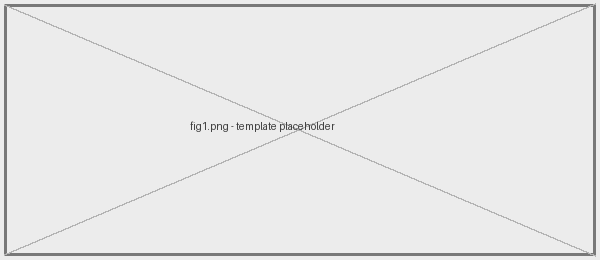
\includegraphics{fig1.png}}
\caption{Example of a figure caption.}
\label{fig}
\end{figure}

Figure Labels: Use 8 point Times New Roman for Figure labels. Use words
rather than symbols or abbreviations when writing Figure axis labels to
avoid confusing the reader. As an example, write the quantity
``Magnetization'', or ``Magnetization, M'', not just ``M''. If including
units in the label, present them within parentheses. Do not label axes only
with units. In the example, write ``Magnetization (A/m)'' or ``Magnetization
\{A[m(1)]\}'', not just ``A/m''. Do not label axes with a ratio of
quantities and units. For example, write ``Temperature (K)'', not
``Temperature/K''.

\section*{Acknowledgment}

The preferred spelling of the word ``acknowledgment'' in America is without
an ``e'' after the ``g''. Avoid the stilted expression ``one of us (R. B.
G.) thanks $\ldots$''. Instead, try ``R. B. G. thanks$\ldots$''. Put sponsor
acknowledgments in the unnumbered footnote on the first page.

\section*{References}

Please number citations consecutively within brackets \cite{b1}. The
sentence punctuation follows the bracket \cite{b2}. Refer simply to the reference
number, as in \cite{b3}---do not use ``Ref. \cite{b3}'' or ``reference \cite{b3}'' except at
the beginning of a sentence: ``Reference \cite{b3} was the first $\ldots$''

Number footnotes separately in superscripts. Place the actual footnote at
the bottom of the column in which it was cited. Do not put footnotes in the
abstract or reference list. Use letters for table footnotes.

Unless there are six authors or more give all authors' names; do not use
``et al.''. Papers that have not been published, even if they have been
submitted for publication, should be cited as ``unpublished'' \cite{b4}. Papers
that have been accepted for publication should be cited as ``in press'' \cite{b5}.
Capitalize only the first word in a paper title, except for proper nouns and
element symbols.

For papers published in translation journals, please give the English
citation first, followed by the original foreign-language citation \cite{b6}.

\begin{thebibliography}{00}
\bibitem{b1} G. Eason, B. Noble, and I. N. Sneddon, ``On certain integrals of Lipschitz-Hankel type involving products of Bessel functions,'' Phil. Trans. Roy. Soc. London, vol. A247, pp. 529--551, April 1955.
\bibitem{b2} J. Clerk Maxwell, A Treatise on Electricity and Magnetism, 3rd ed., vol. 2. Oxford: Clarendon, 1892, pp.68--73.
\bibitem{b3} I. S. Jacobs and C. P. Bean, ``Fine particles, thin films and exchange anisotropy,'' in Magnetism, vol. III, G. T. Rado and H. Suhl, Eds. New York: Academic, 1963, pp. 271--350.
\bibitem{b4} K. Elissa, ``Title of paper if known,'' unpublished.
\bibitem{b5} R. Nicole, ``Title of paper with only first word capitalized,'' J. Name Stand. Abbrev., in press.
\bibitem{b6} Y. Yorozu, M. Hirano, K. Oka, and Y. Tagawa, ``Electron spectroscopy studies on magneto-optical media and plastic substrate interface,'' IEEE Transl. J. Magn. Japan, vol. 2, pp. 740--741, August 1987 [Digests 9th Annual Conf. Magnetics Japan, p. 301, 1982].
\bibitem{b7} M. Young, The Technical Writer's Handbook. Mill Valley, CA: University Science, 1989.
\end{thebibliography}
\vspace{12pt}
\color{red}
IEEE conference templates contain guidance text for composing and formatting conference papers. Please ensure that all template text is removed from your conference paper prior to submission to the conference. Failure to remove the template text from your paper may result in your paper not being published.

\end{document}
